\documentclass[11pt,]{article}
\usepackage[left=1in,top=1in,right=1in,bottom=1in]{geometry}
\newcommand*{\authorfont}{\fontfamily{phv}\selectfont}
\usepackage[]{mathpazo}


  \usepackage[T1]{fontenc}
  \usepackage[utf8]{inputenc}



\usepackage{abstract}
\renewcommand{\abstractname}{}    % clear the title
\renewcommand{\absnamepos}{empty} % originally center

\renewenvironment{abstract}
 {{%
    \setlength{\leftmargin}{0mm}
    \setlength{\rightmargin}{\leftmargin}%
  }%
  \relax}
 {\endlist}

\makeatletter
\def\@maketitle{%
  \newpage
%  \null
%  \vskip 2em%
%  \begin{center}%
  \let \footnote \thanks
    {\fontsize{18}{20}\selectfont\raggedright  \setlength{\parindent}{0pt} \@title \par}%
}
%\fi
\makeatother




\setcounter{secnumdepth}{3}

\usepackage{longtable,booktabs}

\usepackage{graphicx,grffile}
\makeatletter
\def\maxwidth{\ifdim\Gin@nat@width>\linewidth\linewidth\else\Gin@nat@width\fi}
\def\maxheight{\ifdim\Gin@nat@height>\textheight\textheight\else\Gin@nat@height\fi}
\makeatother
% Scale images if necessary, so that they will not overflow the page
% margins by default, and it is still possible to overwrite the defaults
% using explicit options in \includegraphics[width, height, ...]{}
\setkeys{Gin}{width=\maxwidth,height=\maxheight,keepaspectratio}

\title{Título\\
Subtítulo\\
Subtítulo  }



\author{\Large Darihana Linares Laureano\vspace{0.05in} \newline\normalsize\emph{Estudiante de Lic. en Geografía Mención Recursos Naturales y Ecoturismo,
Universidad Autónoma de Santo Domingo (UASD)}  }


\date{}

\usepackage{titlesec}

\titleformat*{\section}{\normalsize\bfseries}
\titleformat*{\subsection}{\normalsize\itshape}
\titleformat*{\subsubsection}{\normalsize\itshape}
\titleformat*{\paragraph}{\normalsize\itshape}
\titleformat*{\subparagraph}{\normalsize\itshape}

\titlespacing{\section}
{0pt}{36pt}{0pt}
\titlespacing{\subsection}
{0pt}{36pt}{0pt}
\titlespacing{\subsubsection}
{0pt}{36pt}{0pt}





\newtheorem{hypothesis}{Hypothesis}
\usepackage{setspace}

\makeatletter
\@ifpackageloaded{hyperref}{}{%
\ifxetex
  \PassOptionsToPackage{hyphens}{url}\usepackage[setpagesize=false, % page size defined by xetex
              unicode=false, % unicode breaks when used with xetex
              xetex]{hyperref}
\else
  \PassOptionsToPackage{hyphens}{url}\usepackage[unicode=true]{hyperref}
\fi
}

\@ifpackageloaded{color}{
    \PassOptionsToPackage{usenames,dvipsnames}{color}
}{%
    \usepackage[usenames,dvipsnames]{color}
}
\makeatother
\hypersetup{breaklinks=true,
            bookmarks=true,
            pdfauthor={Darihana Linares Laureano (Estudiante de Lic. en Geografía Mención Recursos Naturales y Ecoturismo,
Universidad Autónoma de Santo Domingo (UASD))},
             pdfkeywords = {Geomorfología fluvial, Morfometria de cuencas},  
            pdftitle={Título\\
Subtítulo\\
Subtítulo},
            colorlinks=true,
            citecolor=blue,
            urlcolor=blue,
            linkcolor=magenta,
            pdfborder={0 0 0}}
\urlstyle{same}  % don't use monospace font for urls

% set default figure placement to htbp
\makeatletter
\def\fps@figure{htbp}
\makeatother

\usepackage{pdflscape} \newcommand{\blandscape}{\begin{landscape}}
\newcommand{\elandscape}{\end{landscape}}


% add tightlist ----------
\providecommand{\tightlist}{%
\setlength{\itemsep}{0pt}\setlength{\parskip}{0pt}}

\begin{document}
	
% \pagenumbering{arabic}% resets `page` counter to 1 
%
% \maketitle

{% \usefont{T1}{pnc}{m}{n}
\setlength{\parindent}{0pt}
\thispagestyle{plain}
{\fontsize{18}{20}\selectfont\raggedright 
\maketitle  % title \par  

}

{
   \vskip 13.5pt\relax \normalsize\fontsize{11}{12} 
\textbf{\authorfont Darihana Linares Laureano} \hskip 15pt \emph{\small Estudiante de Lic. en Geografía Mención Recursos Naturales y Ecoturismo,
Universidad Autónoma de Santo Domingo (UASD)}   

}

}








\begin{abstract}

    \hbox{\vrule height .2pt width 39.14pc}

    \vskip 8.5pt % \small 

\noindent Resumen del manuscrito


\vskip 8.5pt \noindent \emph{Keywords}: Geomorfología fluvial, Morfometria de cuencas \par

    \hbox{\vrule height .2pt width 39.14pc}



\end{abstract}


\vskip 6.5pt


\noindent  \section{Introducción}\label{introducciuxf3n}

Desde hace siglos atrás el hombre ha buscado la manera de explicar y
entender las distintas formas que el paisaje terrestre (relieve) posee.
Autores numerosos han investigado la génesis de estas nociones
geomorfológicas, remontándose a tres siglos atrás. Autores como Hutton,
Playfair y Lyell, sirvieron de antecesores o bases para la ciencia
geomorfológica. Tras su consolidación como ciencia en Francia numerosos
autores fueron demostrando la importancia de esta ciencia, incluso
ramificándola (climática, eólica, litoral, glaciar, estructural,
tectónica, kárstica y fluvial; siendo la última de interés para esta
investigación), para mayor eficacia en sus estudios.

Los estudios en la geomorfología fluvial a nivel mundial son numerosos y
han servido para explicar cómo los drenajes de los ríos y sus redes
hidrográficas son importantes para la geomorfología, ya que estas redes
fluviales son parte de los procesos de modelado más activos en la
formación del relieve y que permiten mensurar la configuración del
mismo. Para los estudios en geomorfología fluvial, se hace uso del
análisis morfométrico de cuencas hidrográficas. La morfometría de cuenca
se ha convertido en la técnica cuantitativa para el estudio de las
cuencas de manera detallada y ordenada. Actualmente en la República
Dominicana el uso del análisis morfométrico para estudiar cuencas
hidrográficas es poco e insuficiente, a pesar de que la República
Dominicana goza de una diversa y extensa red de cuencas hidrográficas,
ricas y aprovechables para la aplicación de diversas técnicas con el fin
de explicar y entender las propiedades del relieve y su relación con las
cuencas fluviales. Por lo que, este estudio es un aporte para dar a
conocer la configuración y modelado de la cuenca hidrográfica del rio
Guayubín, con el fin de fijar parámetros que permitan evaluar esta
cuenca fluvial; identificando el aspecto general de la cuenca y de la
red, el orden de red y análisis hortoniano, los perfiles longitudinales
e índice de concavidad de cursos más largos, y la morfometría de cuenca.
En ese mismo orden es imprescindible conocer el concepto de cuenca
fluvial o de drenaje, que no es más que el conjunto de cuerpos de agua
con un área determinada que fluyen por distintos canales y escurren en
un mismo desagüe. Según los autores Gregory y Walling, 1973; y Chorley,
1969 (como citó Gutiérrez Elorza (2008)), una cuenca fluvial compone el
espacio determinado en el que se suministran las aguas que discurren por
la superficie, el mismo está delimitado tanto por su relieve y su
hidrología. También considerada como una unidad imprescindible en
geomorfológica.

\subsection{Revisión bibliográfica}\label{revisiuxf3n-bibliogruxe1fica}

Aspecto general de la cuenca y de la red

El aspecto general de la cuenca y de la red se refiere a los parametros
hidrogrñaficos que posee la cuenca (la acumulación de flujos y cálculo
de su umbral, elevación, depresión, y otros). Según Castillo (2015), la
acumulación de flujos señala a todas las celdas que desaguan en una en
particular, la misma se adquiere partiendo de la dirección de la
corriente o flujo. Venkatachalam et al. (2001) dicen que la acumulación
de flujo de una celda se instituye de acuerdo a la sumatoria de los
valores de la acumulación de flujo de las celdas proximas que drenan en
ella.En cuanto al umbral, según ESRI (2012), se es necesario un raster
de acumulación de flujo y la `porción mínima de celdas que componen una
corriente de agua. También se refiere a la forma que adquiere la cuenca
y a la forma de su red de drenaje, según la conformación de sus ríos y
el material rocoso que la compone (patrones de drenaje). Varios autores
expresan que existe una conexión entre la estructura que posee la red de
drenaje con el material rocoso (Pedraza Gilsanz (1996), Gutiérrez Elorza
(2008), Howard (1967), Gregory \& Walling (1973)).

Orden de red y análisis hortoniano

El orden de red hace referencia al orden en el que se clasifican los
cursos de agua, todo en base a su ramificación. Según Wikipedia (2020),
el orden de un curso de agua es siempre un número entero positivo que se
usa tanto en Geomorfología como en Hidrología para denotar la magnitud
de ramificación que posee una red fluvial. Para Bowden \& Wallis (1964),
el orden de red sostiene una relación entre las rocas con la
configuración de la red fluvial y con los procesos tanto hidrológicos
como erosivos. La clasificación de la red se hace de manera jerárquica.
Hoy día existen múltiples normas para determinar la jerarquía de una
red: Strahler (1952), Horton (1945), Shreve (1967), Scheidegger (1970),
Leopold et al. (1964) Hack (1957) y Topological.

Dice Pinilla (1993) que para los años 40 el análisis hortoniano habia
sentado las bases de lo que hoy es la morfometría fluvial; por lo que la
aplicación del analisis hortoniano al estudio de cuencas hidrográficas
son imprecindibles. Para Horton (1945), la razón de bifurcación resulta
ser la conexión entre el número de redes fluviales de una jerarquía
asignada entre el número de redes de jerarquía mayor próxima.

Perfiles longitudinales e índice de concavidad de cursos más largos

El perfil longitudinal de un curso de agua es una línea adquirida al
representar las diversas alturas que se presentan desde el nacimiento de
este hasta donde desagua (Gutiérrez Elorza (2008)). Según Pedraza
Gilsanz (1996), por medio de los perfiles longitudinales es posible
fundamentar definiciones en segmentos con geometría heterogénea
(cóncavo, convexo y rectilíneo), o pendiente; las acomodaciones para
cada parte a una función matematica; e incluso análisis geométricos
basados en elementos físicos o evolutivos. Gutiérrez Elorza (2008), dice
que el perfil longitudinal es generalmente cóncavo, aunque esta
concavidad no está clara para muchos cursos fluviales. En cuanto al
índice de concavidad, este no es más que un indicador que hace posible
la evaluación del nivel de torcedura o curvatura del perfil longitudinal
(Garzón Heydt, Ortega, Garrote, \& others (n.d.)). Se calcula así, la
superficie debajo del perfil longitudinal es extraída del total del área
debajo del segmento que conecta los dos límites del perfil (Goldrick \&
Bishop (2007)).

Morfometría de cuenca

El análisis morfométrico abarca un conjunto de índices morfológicos que
apuntan a un análisis detallado y cuantitativo de cuencas hidrográficas
(Morais \& Almeida (2010)). El análisis morfométrico de cuencas
hidrográficas se inicia por la ordenación de canales fluviales, con la
finalidad de establecer una jerarquía fluvial. Esta, a su vez, consiste
en el proceso de establecer la clasificación de determinado curso de
agua (o el área drenada que le pertenece) en el conjunto total de la
cuenca hidrográfica en la que se encuentra. Aunque, según el autor, esto
se logra con la función de facilitar y volver más objetivos los estudios
morfométricos sobre las cuencas hidrográficas (Christofoletti (1988)).
En cuanto a la curva hipsométrica de una cuenca Strahler (1952) dice que
el porcentaje de la curva hipsométrica no es mas que la relación entre
el área de la sección diagonal horizontal de una red de drenaje con una
altitud relativa sobre la boca de la cuenca, e incluso estas curvas
pueden ser explicadas y relacionadas a través del uso de parámetros
bidimensionales. Y referenter a la integral Hipsométrica, Fernandez \&
Rocha (2016) expresa que el cálculo de este índice mide como está
distribuida la altitud del en una cuenca fluvial.

Este estudio proporciona nueva información sobre la cuenca del río
Guayubín en el campo de Morfometría fluvial, sabiendo que este es el
primer estudio morfométrico que se realiza a la cuenca; y además este
posee un script el cual permite su reproducción sin coste alguno. En
específico, se indaga en el aspecto general de la cuenca y de la red, el
umbral de acumulación de flujo en numero de celdas, la forma que posee
la cuenca y su red de drenaje, considerando la relación que tiene la
forma de la cuenca y la forma de su red de drenaje con el material
rocoso y el relieve (hidrología-topografía-litología). También, en el
orden de red y la implementación del analisis hortoniano se tiene
interes en la forma en la que se organiza o clasifica el orden de red
asignado a cada curso fluvial en la cuenca, así como la razón de
bifurcación de los órdenes de red fluvial. En cuanto a los perfiles
longitudinales y sus indices de concavidad se estudia la geometría que
posee cada segmento de los cursos, en este caso el de los más largos;
tomando en consideración las diversas alturas presentes en el curso. Y,
por último, nos interesa examinar la cuenca de forma cuantitativa, para
conocer sus medidas básicas (área, perímetro, numero de orden de redes,
pendiente, etc.). El interés de este estudio es indar e interpretar lo
siguiente: rango de umbral de acumulación, forma de la cuenca, forma de
su red de drenaje, fenómenos que pueden afectar a la cuenca, si existe
un patrón en la cuenca acorde a su red drenaje, si existe la relación
litología-perfil longitudinal e índice de concavidad de los cursos de
aguas más largos, y, por último, conocer la relación de las
características litológicas y estructurales de la cuenca.

\section{Área de estudio}\label{uxe1rea-de-estudio}

La cuenca del río Guayubín se encuentra entre las morforegiones
Cordillera Central y Valle del Cibao Occidental, en la República
Dominicana (latitud 19.46\(^\circ\)N, longitud -71.41\(^\circ\)W), entre
las provincias Santiago Rodríguez, Monte Cristi y Dajabón. En la
provincia Dajabón engloba de forma completa el municipio El Pino, y de
manera parcial los municipios Loma de Cabrera y Partido; en la provincia
Monte Cristi contiene parcialmente los municipios Las Matas de Santa
Cruz y Guayubín; y en la provincia Santiago Rodríguez comprende los
municipios Villa Los Almácigos y San Ignacio de Sabaneta. Los
munipicpios más poblados en el interior de la cuenca son Guayubín
(35,923 hab.), San Ignacio de Sabaneta (34,540 hab.), y Loma de Cabrera
(15,624 hab.). (ver figura \ref {mapacuenca})

La cuenca del río Guayubín, según Medio Ambiente y Recurso Naturales
(2015), abarca una área de 770.35 km\textsuperscript{2}. De acuerdo con
el mapa de Medio Ambiente y Recurso Naturales (2015), la cabecera del
rio Guayubín se ubica en la vertiente noroeste de el Cerro La Pelada, en
un paraje denominado Palo Amarillo; mientras que sus aguas se vierten en
el río Yaque del Norte, localidad Guayubín.
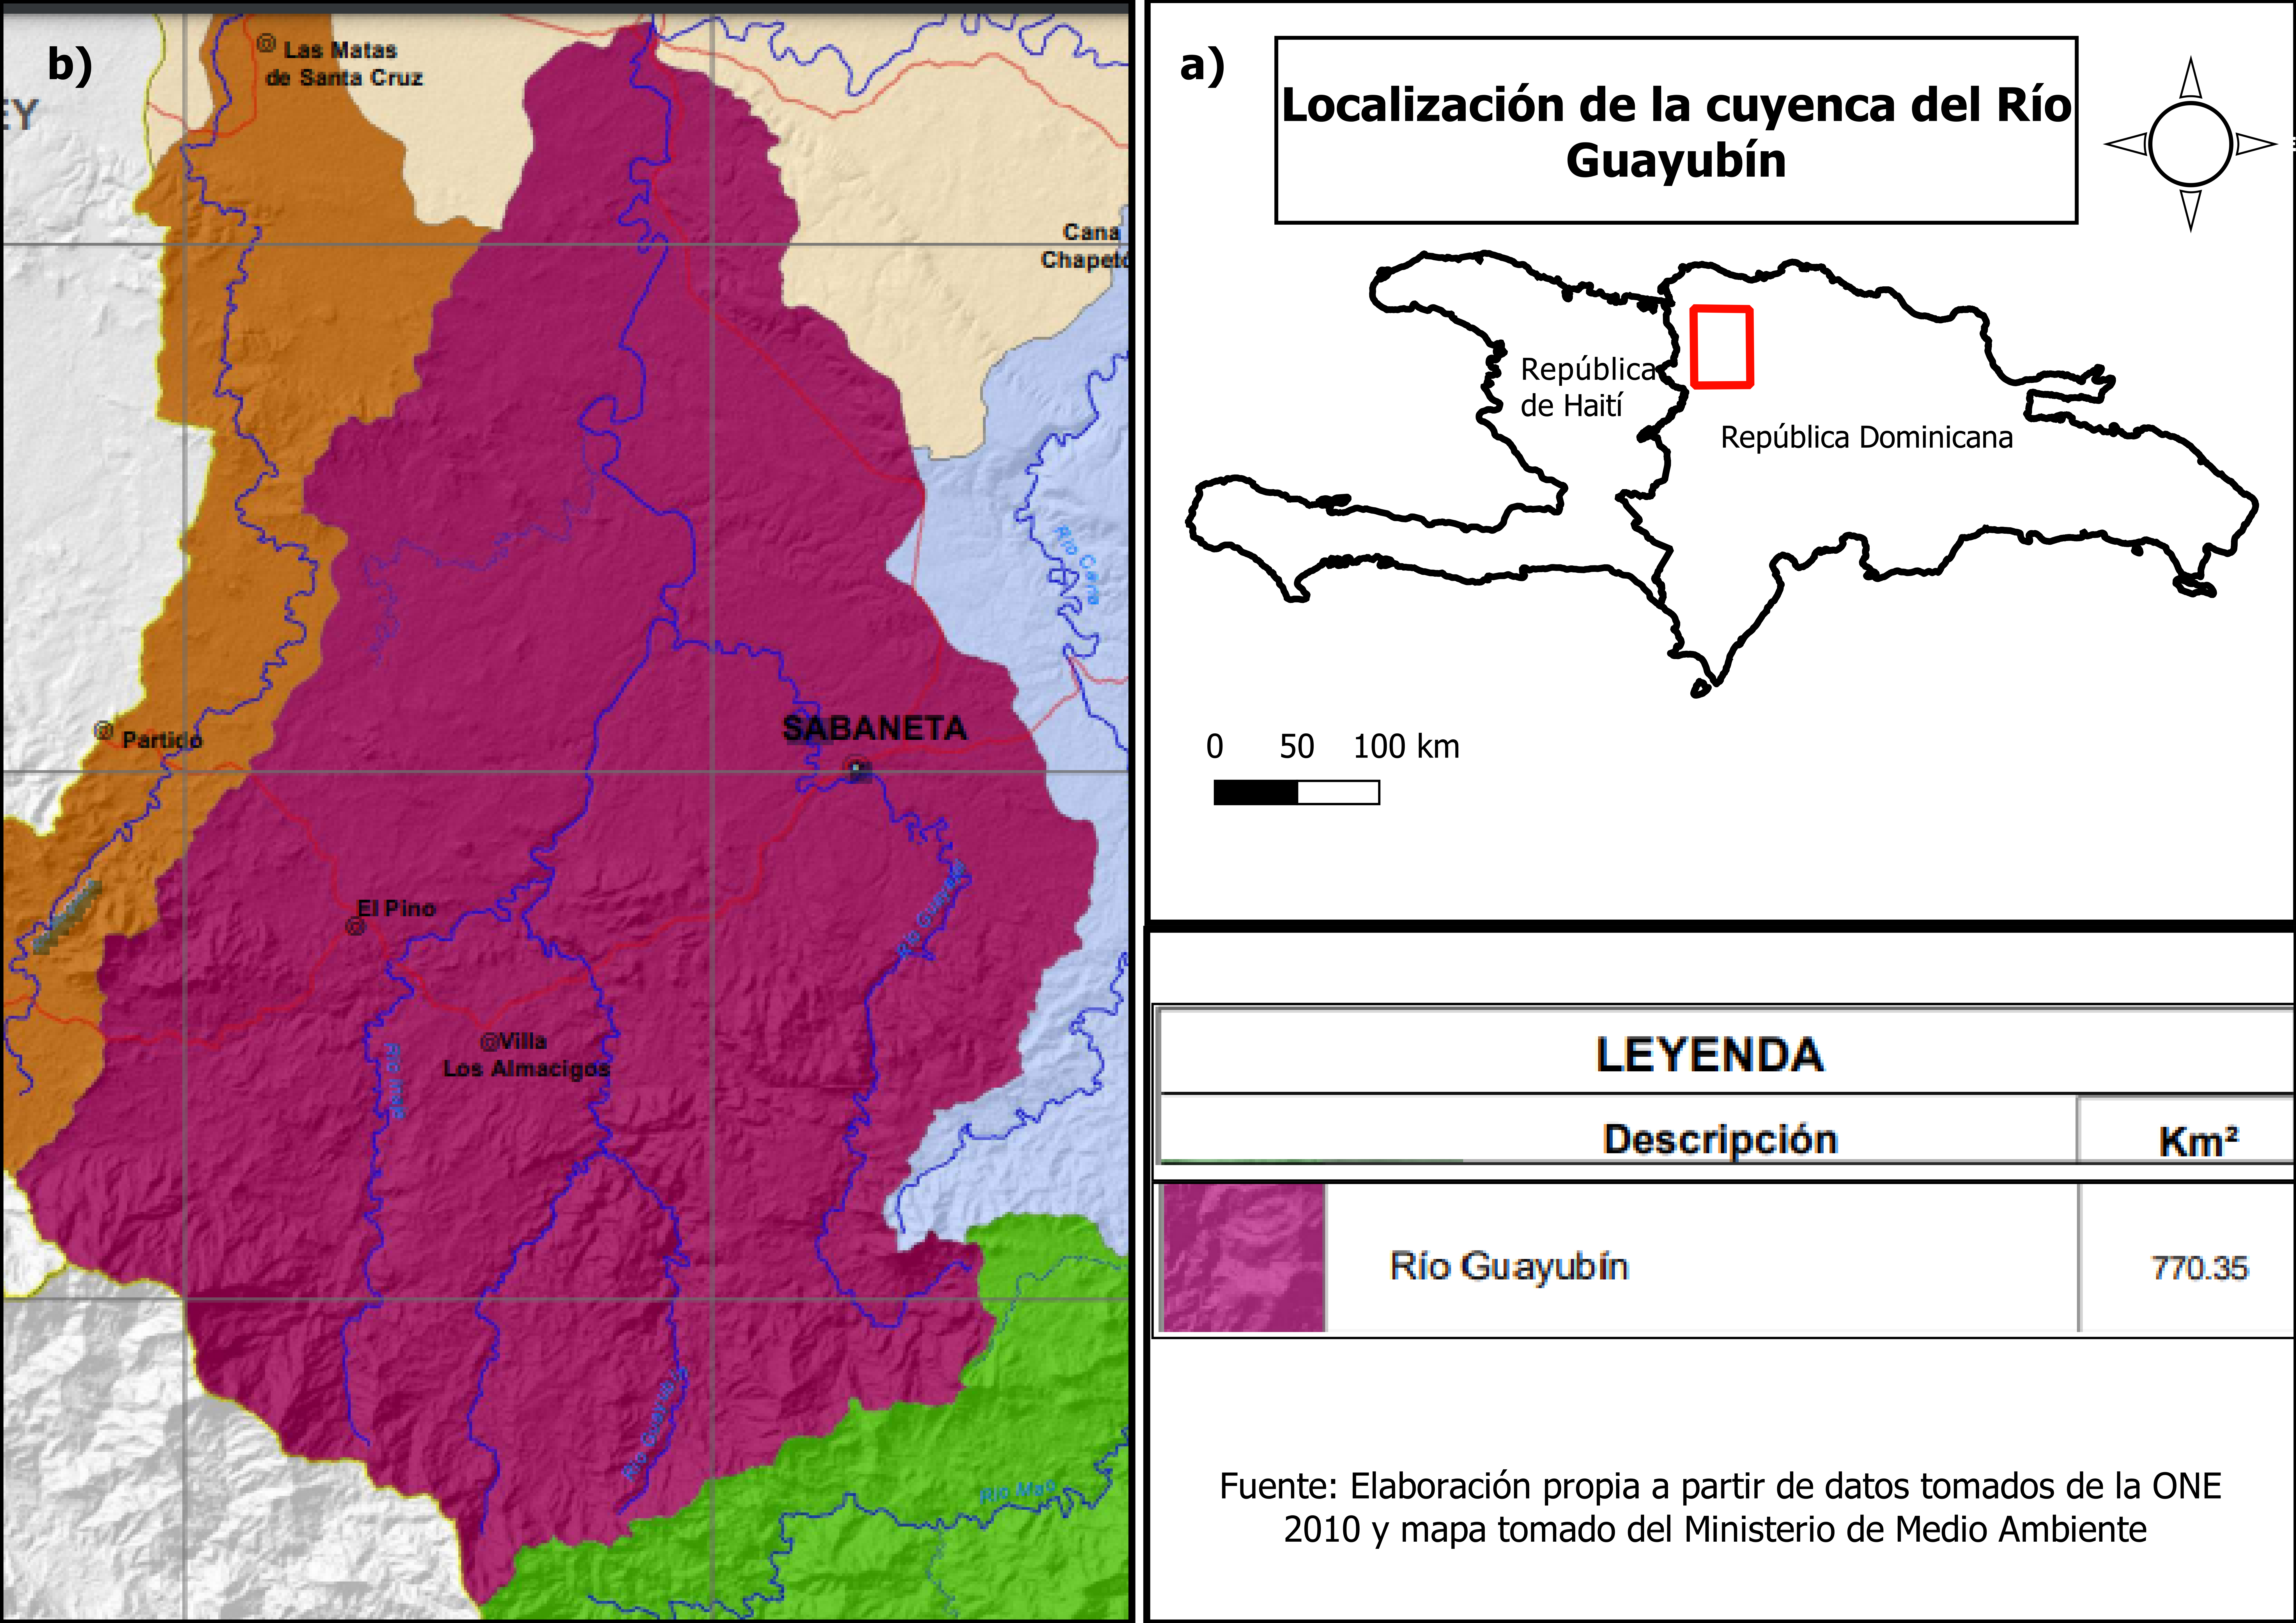
\includegraphics[width=0.90000\textwidth]{Mapa final.png}

\section{Materiales y Metodología}\label{materiales-y-metodologuxeda}

Para el estudio morfométrico de la cuenca Guayubín se usó softwares de
código abierto como medio para procesar datos estadísticos y modelos
digitales con la finalidad de generar las informaciones ha analizar e
interpretar.

\subsection{Materiales}\label{materiales}

\begin{longtable}[]{@{}cc@{}}
\toprule
\begin{minipage}[b]{0.11\columnwidth}\centering\strut
Materiales\strut
\end{minipage} & \begin{minipage}[b]{0.83\columnwidth}\centering\strut
Uso\strut
\end{minipage}\tabularnewline
\midrule
\endhead
\begin{minipage}[t]{0.11\columnwidth}\centering\strut
RStudio\strut
\end{minipage} & \begin{minipage}[t]{0.83\columnwidth}\centering\strut
donde se redactó el manuscrito, se procesaron los datos que ofrece el
DEM de la cuenca a traves de un script en el que se usaron paquetes que
produjeran los resultados.\strut
\end{minipage}\tabularnewline
\begin{minipage}[t]{0.11\columnwidth}\centering\strut
library rgrass7\strut
\end{minipage} & \begin{minipage}[t]{0.83\columnwidth}\centering\strut
es una interfaz que permite establecer una conexión entre la version 7
del sistema de infromacion geográfica GRASS, y R, que crea un entorno
GRASS desechable dentro de R.\strut
\end{minipage}\tabularnewline
\begin{minipage}[t]{0.11\columnwidth}\centering\strut
library sp\strut
\end{minipage} & \begin{minipage}[t]{0.83\columnwidth}\centering\strut
este paquete sirve para la importación, manipulación y exportación de
datos espaciales en R, y para métodos que incluyen imprimir / mostrar,
trazar, entre otros.\strut
\end{minipage}\tabularnewline
\begin{minipage}[t]{0.11\columnwidth}\centering\strut
library sf\strut
\end{minipage} & \begin{minipage}[t]{0.83\columnwidth}\centering\strut
crea caracteristicas simples (simple features), que amplían los objetos
tipo data.frame con una columna de lista de características
simples.\strut
\end{minipage}\tabularnewline
\begin{minipage}[t]{0.11\columnwidth}\centering\strut
library raster\strut
\end{minipage} & \begin{minipage}[t]{0.83\columnwidth}\centering\strut
este paquete proporciona clases y funciones para manipular datos
geográficos (espaciales) en formato `ráster'.\strut
\end{minipage}\tabularnewline
\begin{minipage}[t]{0.11\columnwidth}\centering\strut
library leaflet\strut
\end{minipage} & \begin{minipage}[t]{0.83\columnwidth}\centering\strut
esta función crea un widget de mapa de folletos utilizando htmlwidgets.
El widget se puede representar en páginas HTML generadas a partir de R
Markdown, y otros.\strut
\end{minipage}\tabularnewline
\begin{minipage}[t]{0.11\columnwidth}\centering\strut
library leafem\strut
\end{minipage} & \begin{minipage}[t]{0.83\columnwidth}\centering\strut
es un paquete que provee una extensión para leaflet uasados para
paquetes mapview, permite mostrar las coordenadas de la posición del
puntero del mouse, consultar valores de imagen a través de puntero del
mouse y botones de zoom a capa.\strut
\end{minipage}\tabularnewline
\begin{minipage}[t]{0.11\columnwidth}\centering\strut
library mapview\strut
\end{minipage} & \begin{minipage}[t]{0.83\columnwidth}\centering\strut
el paquete proporciona funcionalidad para ver objetos espaciales de
forma interactiva.\strut
\end{minipage}\tabularnewline
\begin{minipage}[t]{0.11\columnwidth}\centering\strut
library readr\strut
\end{minipage} & \begin{minipage}[t]{0.83\columnwidth}\centering\strut
el objetivo de `readr' es proporcionar una forma rápida y amigable de
leer datos rectangulares (como `csv', `tsv' y `fwf').\strut
\end{minipage}\tabularnewline
\begin{minipage}[t]{0.11\columnwidth}\centering\strut
QGIS with GRASS\strut
\end{minipage} & \begin{minipage}[t]{0.83\columnwidth}\centering\strut
para la visualización de vectores y rasters generados con RStudio en una
región de GRASS,como la visualización de los mapas Topológicos y
Geológicos de la República Dominicana, tambien, para la creación de
algunos mapas de localización.\strut
\end{minipage}\tabularnewline
\begin{minipage}[t]{0.11\columnwidth}\centering\strut
Google Earth\strut
\end{minipage} & \begin{minipage}[t]{0.83\columnwidth}\centering\strut
para observar datos en formato kml generados y exportados de RStudio y
asi como la representacion del relieve del lugar de estudio.\strut
\end{minipage}\tabularnewline
\begin{minipage}[t]{0.11\columnwidth}\centering\strut
Mapa Topológico de RD\strut
\end{minipage} & \begin{minipage}[t]{0.83\columnwidth}\centering\strut
para hacer comparaciones y obtener referencias sobre el relieve.\strut
\end{minipage}\tabularnewline
\begin{minipage}[t]{0.11\columnwidth}\centering\strut
Mapa Geológico Nacional de RD\strut
\end{minipage} & \begin{minipage}[t]{0.83\columnwidth}\centering\strut
para hacer comparaciones y obtener referencias sobre la composición
rocosa y los años que datan estas.\strut
\end{minipage}\tabularnewline
\bottomrule
\end{longtable}

\subsection{Metodología}\label{metodologuxeda}

Aspecto de la cuenca y de la red de drenaje. Los parametros de la cuenca
fueron calculados por medio de el addon de GRASS GIS
\texttt{r.watershed} (Charles Ehlschlaeger (2003--2021b)), utilizando un
Dem , los parametros calculados fueron acumulación, elevación,
depresión, drenaje, flujo, cuenca y media cuenca, con un umbral de
acumulación de flujo de 80 celdas necesarias para que exista una red de
agua.

Se usó el addon \texttt{r.water.outlet} (Charles Ehlschlaeger
(2003--2021a)) para la extraccion de la cuenca a traves de un mapa de
direccion de drenajes (creado con el addon \texttt{r.watershed}), y de
coordenadas de desembocadura de la cuenca (obtenidas con
\texttt{Mapview}). Asi tambien, se usó el addon \texttt{r.to.vect} (Team
(2003--2021)), para convertir un raster en vectorial.

Para estraer la red de drenaje se hizo uso de el addon
\texttt{r.stream.extract} (Metz (2003--2021)), donde se utilizo un
raster como capa de entrada y se genero un archivo en formato vectorial,
ademas, del raster, es necesario el umbral de acumulación de flujo.

En cuanto al orden de red y el analisis hortoniano, se usó el addon
\texttt{r.stream.extract} (Metz (2003--2021)), para producir un mapa de
dirección de flujo el cual sirvió para la creación de mapas de ordenes
de redes generados con \texttt{r.stream.order} (Jasiewicz (2003--2021)).
Además de el mapa de direccion de flujo, se uso un raster de red de la
cuenca, flujo de acumulacion y un modelo de elevacion. Se calcularon los
ordenes de redes segun las clasificaciones de Strahler, Horton, Shreve,
Hack y Topo, pero, se uso la red de orden segun Strahler para delimitar
la cuenca. Mientras que se usaron los addons \texttt{r.info} para
obtener los valores minimos y maximos del orden de red segun Strahler;
para delimitar la cuenca a traves de la red de drenaje se utilizo
\texttt{r.stream.basins} (Jarek Jasiewicz \& Institute (2003--2021a)); y
para calcular las estadisticas de red de Horton ordenadas para redes de
orden de Strahler y Horton se uso \texttt{r.stream.stats} (Jarek
Jasiewicz \& Institute (2003--2021b)).

Para calcular los indices de concavidad y los perfiles longitudinales,
primero, se obtuvieron los cursos mas largos de la cuenca a traves de la
funcion \texttt{LfpNetwork} (Batlle (2018b)), usando coordenadas de
desembocadura de la cuenca obtenidas con \texttt{Mapview}, vectores de
ordenes de red y mapa de flujo de direccion. Segundo, para producir los
perfiles longitudinales e indices de cocavidad se empleo la funcion
\texttt{LfpProfilesConcavity} (Batlle (2018c)), utilizando la red de
cursos de agua mas largos, coordenadas de desembocadura, un dem y un
mapa de flujos de drenaje.

Para la obtencion de los parametros morfometricos de la cuenca se uso el
addon \texttt{r.basin} (Margherita Di Leo (2003--2021)), por medio de un
modelo de elevacion y coordenadas proyectadas de la salida de la cuenca,
obtenidas en geograficas con \texttt{Mapview} y transformadas a
proyectadas con la funcion \texttt{My\_Trans} (Batlle (2020)).

Respecto al cálculo de la curva e integral hipsométrica, se utilizó la
función \texttt{HypsoIntCurve} (Batlle (2018a)), a través de vectores de
arroyos de cuenca de orden 2 y 3.

\section{Resultados}\label{resultados}

Aspecto general de la cuenca y de la red de drenaje. Tras cálcular los
parámetros hidrograficos de la cuenca con \texttt{r.watershed} se obtuvo
tres grupos de capas (DEM, basins y str), que con la ayuda de
\texttt{leaflet} se generó un mapa que muestra las subcuencas, las redes
fluviales y el DEM, de la cuenca sin delimitar. La cuenca extraida con
\texttt{r.water.outlet} produjo un raster de cuenca delimitada que se
transformó a vector con \texttt{r.to.vect}. En cuanto a la red de
drenaje extraida con \texttt{r.stream.extract} se generó un raster y un
vector con redes fluviales formadas a partir de un umbral de 80 celdas.

Orden de red analisis hortoniano Con \texttt{r.stream.extract} se
crearon mapas basados en las clasificaciones de Strahler, Horton,
Shreve, Hack y Topo. Se ordenó y clasificó cada tramo fluvial de la
cuenca según Strahler donde el orden máximo de red es 5 y el minimo es
de 1. Según la clasificación de Strahler usada para analizar la red,
obtenidas con \texttt{r.stream.stats}, se produjeron 367 redes fluviales
de las cuales 284 redes eran de orden 1, mientras que de orden 2 se
produjeron 61 redes, 17 redes de orden 3, 4 redes de orden 4, y 1 red de
orden 5. (ver figura\ref {grafnro}).

\begin{figure}
\centering
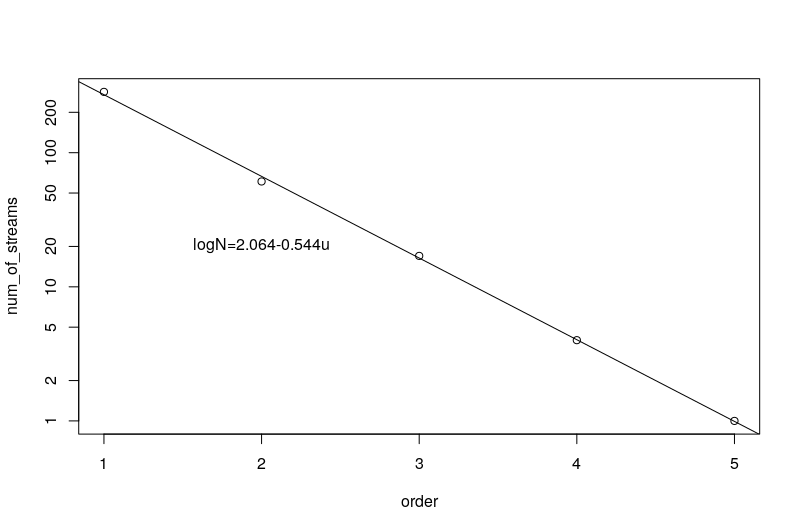
\includegraphics[width=0.80000\textwidth]{Numero de red segun su orden.png}
\caption{Número de redes segun su orden\label{grafnro}}
\end{figure}

En cuanto al área de cuenca resultante de esta operación fue de 773.2235
km\textsuperscript{2}. De manera mas detallada los resultados del area
de cuenca encontrados segun orden de red fueron los siguientes:

\begin{longtable}[]{@{}cc@{}}
\toprule
Orden & Area total (km\textsuperscript{2})\tabularnewline
\midrule
\endhead
1 & 488.1383\tabularnewline
2 & 444.7173\tabularnewline
3 & 539.4576\tabularnewline
4 & 590.9969\tabularnewline
5 & 773.2235\tabularnewline
\bottomrule
\end{longtable}

Mientras que los resultados de la razón de bifurcación obtenidas para de
cada orden de red fueron:

\begin{longtable}[]{@{}cc@{}}
\toprule
Orden & Razón de Bifurcación\tabularnewline
\midrule
\endhead
1 & 4.6557\tabularnewline
2 & 3.5882\tabularnewline
3 & 4.2500\tabularnewline
4 & 4.0000\tabularnewline
5 & 0.0000\tabularnewline
\bottomrule
\end{longtable}

\section{Discusión}\label{discusiuxf3n}

De acuerdo con el s.a. (s.f.), la cabecera del rio Guayubin se ubica en
las inmediaciones de loma escondida

\section{Agradecimientos}\label{agradecimientos}

\section{Información de soporte}\label{informaciuxf3n-de-soporte}

\section{\texorpdfstring{\emph{Script}
reproducible}{Script reproducible}}\label{script-reproducible}

\section*{Referencia}\label{referencia}
\addcontentsline{toc}{section}{Referencia}

\hypertarget{refs}{}
\hypertarget{ref-Hypsocjose}{}
Batlle, J. R. M. (2018a). \emph{Función hypsointcurve}. Retrieved from
\url{https://github.com/geofis/rgrass/blob/master/integral_hypsometric_curve.R}

\hypertarget{ref-lfpnetjose}{}
Batlle, J. R. M. (2018b). \emph{Función lfpnetwork}. Retrieved from
\url{https://github.com/geofis/rgrass/blob/master/lfp_network.R}

\hypertarget{ref-lfpconcajose}{}
Batlle, J. R. M. (2018c). \emph{Función lfpprofilesconcavity}. Retrieved
from
\url{https://github.com/geofis/rgrass/blob/master/lfp_profiles_concavity.R}

\hypertarget{ref-Mytransjose}{}
Batlle, J. R. M. (2020). \emph{Función my-trans}. Retrieved from
\url{https://github.com/geomorfologia-master/unidad-4-asignacion-1-procesos-fluviales/blob/master/my-trans.R}

\hypertarget{ref-bowden1964effect}{}
Bowden, K. L., \& Wallis, J. R. (1964). Effect of stream-ordering
technique on horton's laws of drainage composition. \emph{Geological
Society of America Bulletin}, \emph{75}(8), 767--774.

\hypertarget{ref-castillo2015delimitacion}{}
Castillo, F. A. J. (2015). Delimitación automática de microcuencas
utilizando datos srtm de la nasa. \emph{Enfoque UTE}, \emph{6}(4),
81--97.

\hypertarget{ref-wateroutlet}{}
Charles Ehlschlaeger, U. A. C. E. R. L. (2003--2021a). \emph{Addon
r.water.outlet}. Retrieved from
\url{https://grass.osgeo.org/grass78/manuals/r.water.outlet.html}

\hypertarget{ref-watershedcharles}{}
Charles Ehlschlaeger, U. A. C. E. R. L. (2003--2021b). \emph{Addon
r.watershed}. Retrieved from
\url{https://grass.osgeo.org/grass79/manuals/r.watershed.html}

\hypertarget{ref-christofoletti1988geomorfologia}{}
Christofoletti, A. (1988). \emph{Geomorfologia}. Editora Blucher.

\hypertarget{ref-ESRI2012}{}
ESRI, E. S. R. I. (2012). ArcGIS resources: Definir cuencas
hidrográficas. Retrieved from
\url{https://help.arcgis.com/es/arcgisdesktop/10.0/help/index.html\#//009z00000068000000}

\hypertarget{ref-fernandez2016analise}{}
Fernandez, O. V. Q., \& Rocha, A. S. da. (2016). Análise preliminar da
aplicação da integral hipsométrica à caracterização das unidades de
paisagem na bacia do paraná iii, oeste do paraná. \emph{Anais VIII
SIMPGEO-as Fronteiras Da Ciência Geográfica: Avanços E Possibilidades.
Marechal Cândido Rondon, N. November}, 497--506.

\hypertarget{ref-garzonmorfologia}{}
Garzón Heydt, G., Ortega, J., Garrote, J., \& others. (n.d.).
\emph{Morfología de perfiles de ríos en roca. control tectónico y
significado evolutivo en el bajo guadiana}.

\hypertarget{ref-goldrick2007regional}{}
Goldrick, G., \& Bishop, P. (2007). Regional analysis of bedrock stream
long profiles: Evaluation of hack's sl form, and formulation and
assessment of an alternative (the ds form). \emph{Earth Surface
Processes and Landforms}, \emph{32}(5), 649--671.

\hypertarget{ref-gregory1973drainage}{}
Gregory, K. J., \& Walling, D. E. (1973). \emph{Drainage basin form and
process}.

\hypertarget{ref-gutierrez2008geomorfologia}{}
Gutiérrez Elorza, M. (2008). \emph{Geomorfología}.

\hypertarget{ref-horton1945erosional}{}
Horton, R. E. (1945). Erosional development of streams and their
drainage basins; hydrophysical approach to quantitative morphology.
\emph{Geological Society of America Bulletin}, \emph{56}(3), 275--370.

\hypertarget{ref-howard1967drainage}{}
Howard, A. D. (1967). Drainage analysis in geologic interpretation: A
summation. \emph{AAPG Bulletin}, \emph{51}(11), 2246--2259.

\hypertarget{ref-streambasinsjareck}{}
Jarek Jasiewicz, G., Adam Mickiewicz University, \& Institute, G.
(2003--2021a). \emph{Addon r.stream.basins}. Retrieved from
\url{https://grass.osgeo.org/grass78/manuals/addons/r.stream.basins.html}

\hypertarget{ref-streamstats}{}
Jarek Jasiewicz, G., Adam Mickiewicz University, \& Institute, G.
(2003--2021b). \emph{Addon r.stream.stats}. Retrieved from
\url{https://grass.osgeo.org/grass78/manuals/addons/r.stream.stats.html}

\hypertarget{ref-streamorder}{}
Jasiewicz, J. (2003--2021). \emph{Addon r.stream.order}. Retrieved from
\url{https://grass.osgeo.org/grass78/manuals/addons/r.stream.order.html}

\hypertarget{ref-basinmargherita}{}
Margherita Di Leo, M. D. S. (2003--2021). \emph{Addon r.basin}.
Retrieved from
\url{https://grass.osgeo.org/grass78/manuals/addons/r.basin.html\#morphometric-parameters-of-basin}

\hypertarget{ref-Mmar2015cuenca}{}
Medio Ambiente y Recurso Naturales, M. de. (2015). \emph{Cuenca río
yaque del norte y su zona costera}.
urlhttp://ambiente.gob.do/wp-content/uploads/2016/11/Yaque-del-Norte-Subcuencas-Hidrograficas-1.pdf.

\hypertarget{ref-streamnextractmarkus}{}
Metz, M. (2003--2021). \emph{Addon r.stream.extract}. Retrieved from
\url{https://grass.osgeo.org/grass78/manuals/r.stream.extract.html}

\hypertarget{ref-morais2010geomorfologia}{}
Morais, F., \& Almeida, L. M. (2010). Geomorfologia fluvial da bacia
hidrográfica do ribeirão jaú-palmas-to. \emph{Brazilian Geographical
Journal: Geosciences and Humanities Research Medium}, \emph{1}(2).

\hypertarget{ref-pedraza1996geomorfologia}{}
Pedraza Gilsanz, J. de. (1996). \emph{Geomorfología: Principios, métodos
y aplicaciones}.

\hypertarget{ref-pinilla1993symposium}{}
Pinilla, A. (1993). \emph{Symposium sobre la raña en españa y portugal}
(Vol. 2). Editorial CSIC-CSIC Press.

\hypertarget{ref-strahler1952hypsometric}{}
Strahler, A. N. (1952). Hypsometric (area-altitude) analysis of
erosional topography. \emph{Geological Society of America Bulletin},
\emph{63}(11), 1117--1142.

\hypertarget{ref-tovect}{}
Team, G. D. (2003--2021). \emph{Addon r.to.vect}. Retrieved from
\url{https://grass.osgeo.org/grass76/manuals/r.to.vect.html}

\hypertarget{ref-venkatachalam2001automatic}{}
Venkatachalam, P., Mohan, B., Kotwal, A., Mishra, V., Muthuramakrishnan,
V., \& Pandya, M. (2001). Automatic delineation of watersheds for
hydrological applications proc. \emph{ACRS 2001-22nd asian conference on
remote sensing, 5-9 november 2001, singapore. vol}, \emph{2},
1096--1101.

\hypertarget{ref-wikipedia2020stream}{}
Wikipedia, C. (2020). Stream order. Retrieved from
\url{https://en.wikipedia.org/wiki/Stream_order}




\newpage
\singlespacing 
\end{document}
